\chapter{Proposal} \label{chapter_6}


	This chapter summarises the expected outcomes from this research work along with a proposed timeline for the implementation of the different subtasks that form the part of the work. The current progress towards the development of the Gibbs energy minimiser has also been presented along with a demonstration problem, which is then followed by a brief publication plan.

	
\section{Overall Timeline}
	\begin{table}[!htbp]
		\caption{Overall timeline of the proposed work showing major academic and research milestones.}
		\centering	
  		\begin{tabular}{@{}l r r@{}}
		\toprule
		\multicolumn{1}{c}{\textbf{Item}} & \multicolumn{1}{c}{\textbf{Timeline}} & \multicolumn{1}{c}{\textbf{Status}}\\
		\midrule
		\multicolumn{3}{c}{\textbf{Coursework}}\\
		\midrule
		MCSC-6010G: Mathematical Modelling & Sep. - Dec. 2018 & Complete\\
		MCSC-6030G: High Performance Computing & Sep. - Dec. 2018 & Complete\\
		NUCL-6005G: Computational Thermodynamics [PhD level elective] & Sep. - Dec. 2018 & Complete\\
		MCSC-6020G: Numerical Analysis & Sep. - Dec. 2019 & In progress\\
		\midrule
		\multicolumn{3}{c}{\textbf{Research}}\\
		\midrule
		Literature review of computational thermodynamics and GEM & Sep. - Dec. 2018 & Complete\\
		Implement data file parsing code & Feb. - Mar. 2019 & Complete\\
		Implement linear solver (levelling) & Apr. - Jun. 2019 & Complete\\
		Implement communication between \texttt{Yellowjacket} and \texttt{MOOSE} & Jul. - Aug. 2019 & Complete\\
		Implement non-linear solver for GEM (homogeneous) & Sep. - Dec. 2019 & In progress\\
		Implement non-linear solver for GEM (heterogeneous) & Jan. - Mar. 2020 & Planned\\
		Demonstration of non-linear solver capabilities & Mar. - May 2020 & Planned\\
		Begin integration of thermodynamic solver with \texttt{Marmot} & Jun. - Aug. 2020 & Planned\\ 
		Comparative study of global optimisation strategies & Sep. - Dec. 2020 & Planned\\
		Implementation of global optimisation algorithm & Jan. - Mar. 2021 & Planned\\
		Demonstration of global optimisation capabilities & Apr. - May 2021 & Planned\\
		Complete integration into \texttt{MOOSE} & Jun. - Aug. 2021 & Planned\\
		Verification and testing & Sep. - Dec. 2021 & Planned\\
		\bottomrule
      		\end{tabular}
	\end{table}
	
\section{Current Progress}
	Over the last one year, since starting my PhD at Ontario Tech, significant progress has been made towards the development of the Gibbs energy minimisation code. This includes the development of a robust parser for parsing the data files and the linear solver for initialisation. The current progress in development of the thermodynamic solver for \texttt{Yellowjacket} has been shown in figure~\ref{fig:progress}. The thermochemistry code has been partly integrated with \texttt{MOOSE} and thermochemical equilibrium can be calculated on a \texttt{MOOSE} mesh using the levelling solver. Currently only the ideal mixture phases (denoted with IDMX in ChemSage data files) and the Modified Quasichemical Model (denoted with SUBG in ChemSage data files) for molten salts are supported. These models were selected for the initial development since MQM  are  as the development is underway to expand support to a large number of thermodynamic models.
	
    \begin{figure}[h]
        \centering
        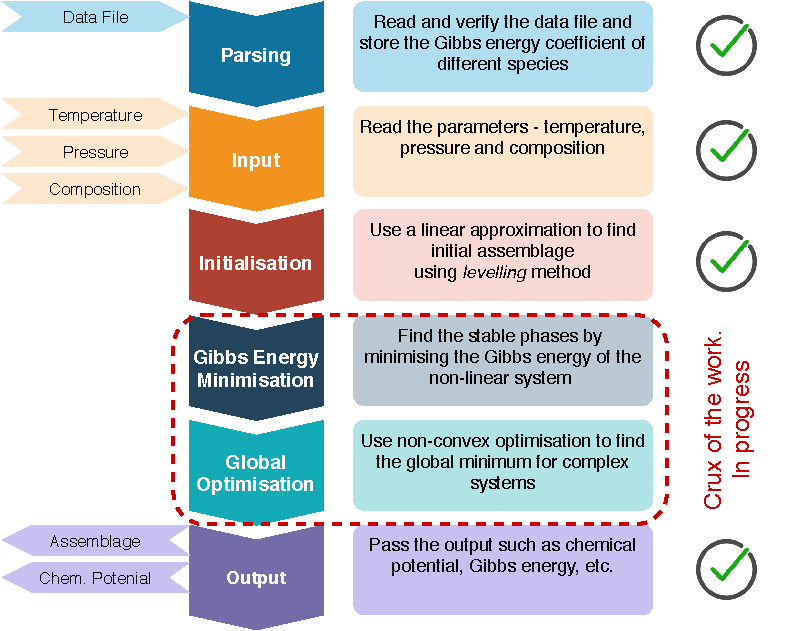
\includegraphics[scale=0.9]{figures/YJ_Progress.pdf}
        \caption{Current progress on the implementation of the thermochemistry solver.}
        \label{fig:progress}
    \end{figure}
	
	It is imperative to advise a word of caution with respect to the progress represented above. While figure~\ref{fig:progress} might make the reader believe that a major part of the work has already been completed, in reality, Gibbs energy minimisation and global optimisation are the major and the most challenging parts of this work and they will be the primary focus over the next year along with expansion of capabilities.
	
	\subsection{Demonstration Problem}
	The reference fuel and coolant proposed for the different MSR concepts are fluoride salts due to their advantageous neutronic and physico-chemical properties \cite{BENES2012359}. \ce{LiF-BeF2} and \ce{LiF-NaF-KF} are amongst the different salt compositions under study for the primary and secondary coolant and their suitability with respect to their corrosion properties for the structural material is an essential requirement for reactor safety and operation. Since \ce{Ni} is the main element for prospective alloys for structural materials, and the rate of corrosion is defined by the redox potential of the molten salt, the phase equilibrium of the salt with potential corrosion products must be studied as a function of temperature and pressure \cite{OcadizFlores18}. Therefore, the initial focus is on \ce{Ni} alloys interacting with molten \ce{LiF2-KF} salts and for the present demonstration the \ce{KF-NiF2} binary system has been selected. This system is not only relevant to the MSR but has also been studied experimentally and the required thermodynamic data is available in literature \cite{OcadizFlores18}.

 	The demonstration problem presented here was a milestone in the first year development plan of \texttt{Yellowjakcte} and was submitted to the Idaho National Lab as part of a progress report. For the demonstration problem, a bar with molar composition \ce{0.8KF + 0.2NiF2} under a temperature gradient as shown in figure~\ref{fig:demo_problem} has been solved for thermodynamic equilibrium using the linear levelling solver.
    
    	\begin{figure}[h]
        		\centering
        		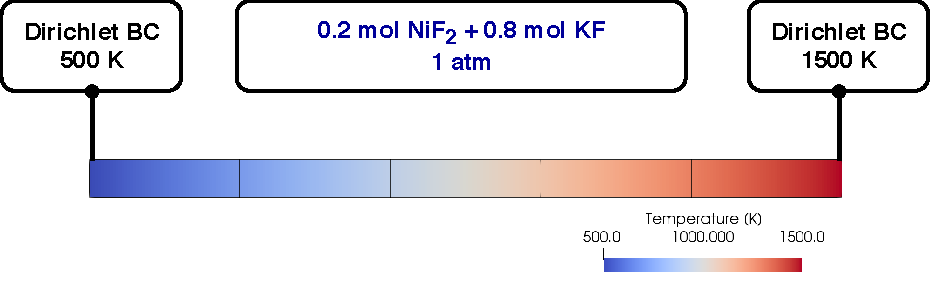
\includegraphics[width=0.75\textwidth]{figures/Demo_prob.pdf}
        		\caption{The demonstration problem consists of a bar divided into 5 elements with Dirichlet boundary conditions imposed at both ends and a linear temperature gradient.}
        		\label{fig:demo_problem}
    	\end{figure}

	\subsection{Results of Demonstration Problem}
	The stable phases and the Gibbs energies predicted by the levelling solver are shown in figure~\ref{fig:results}. As expected from the phase diagram shown below, a transition from a solid phase to a mixture of solid and liquid phase around 1100 \si{\celsius} and a transition from a two-phase region to a single  liquid phase region around 1200 \si{\celsius} is observed.
    
    	\begin{figure}[h]
        		\centering
        		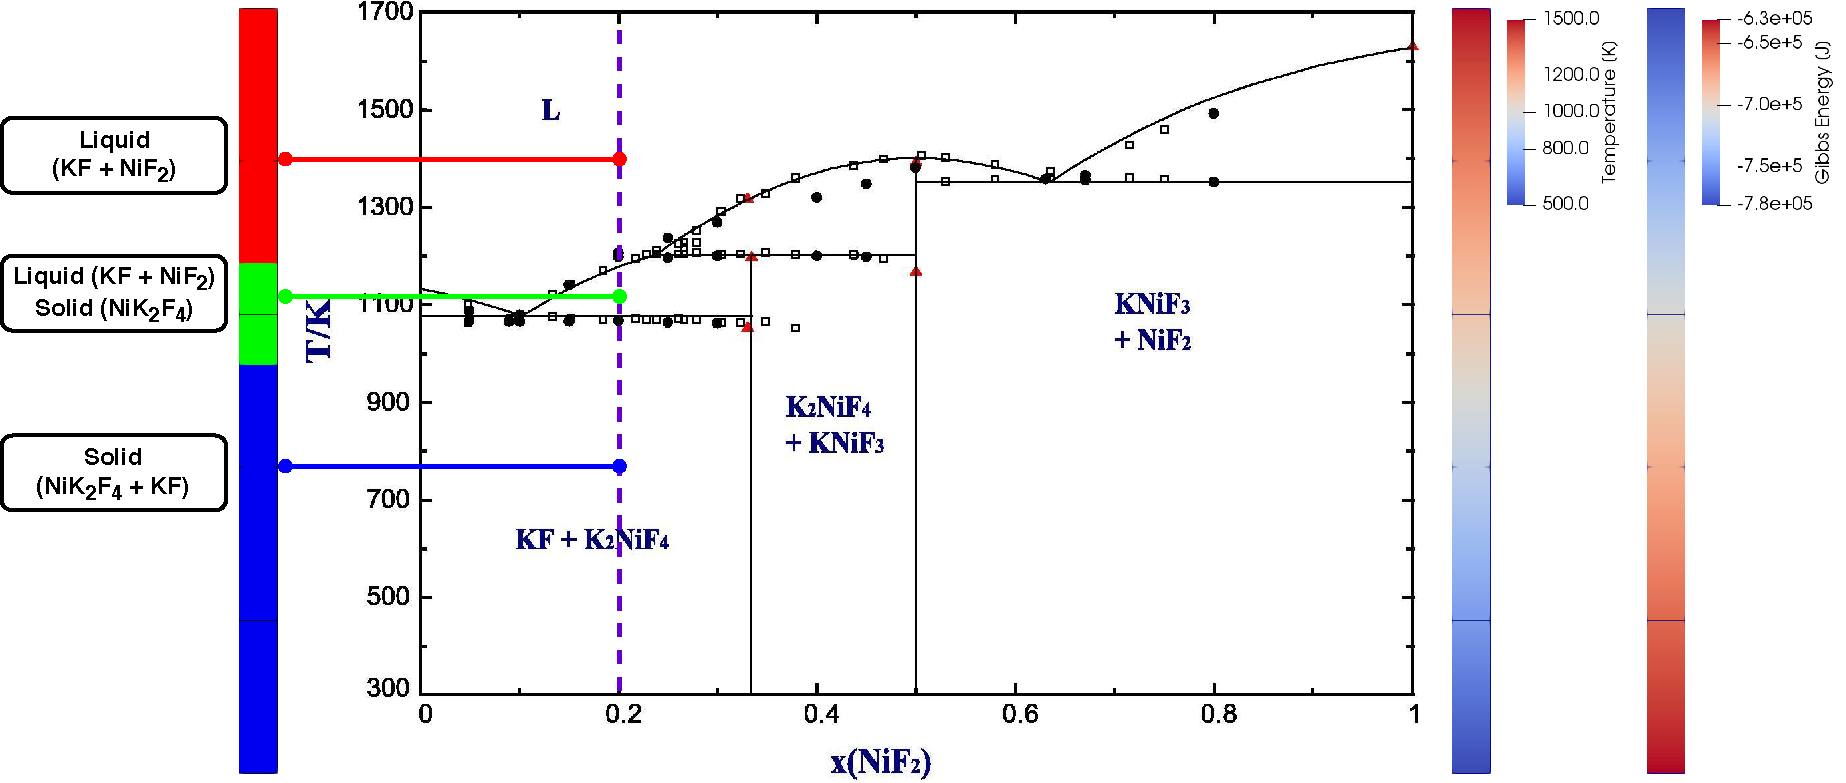
\includegraphics[width=\textwidth]{figures/Results.pdf}
        		\caption{Stable phases and Gibbs energies predicted by the linear solver.}
        		\label{fig:results}
    	\end{figure}

    It must be mentioned that though the Gibbs energy profile shown on the extreme right in figure~\ref{fig:results} is continuous, the actual results on the finite element mesh are discretised due to a step change in the temperature as we move from one element to the other. The continuous profile, has been plotted through \texttt{Paraview}, by interpolation during post processing and is a better representation of the physical conditions where we expect no step changes if a temperature gradient is applied.
    
    It must also be clarified that the in the current state, the under-development thermodynamic solver cannot fully reproduce the phase diagram presented above. The levelling solver coverts all species to ideal phases and therefore any non-linear behaviour (the curved lines on the phase diagram) cannot be reproduced. However, the demonstration problem is successful in showing that the code development is on the correct path and once the non-linear GEM part has been implemented, it will be possible to reproduce the non-ideal behaviour too. 
	
\section{Work Plan} \label{sec:workplan}
	\subsection{Year 2019-2020}
	The primary focus of 2019-2020 will be the implementation of the non-linear solver for thermochemical equilibrium. Using the levelling solver's results as  initial estimates, the non-linear solver will be able to provide the final phase assemblage. Also, the integration of thermodynamic equilibrium code with phase field part of \texttt{Yellowjacket} will be done in the last quarter of 2019-2020.
	\subsubsection{Non-linear solver}
		The implementation of the non-linear solver is relatively straightforward. The implementation of Gibbs energy minimisation method results in system of equations given by equation~\eqref{eq:GEM_mat} and the initial estimates are provided by the levelling solver. The principle tasks in the implementation of the non-linear solver are as as follows:
		\begin{enumerate}
			\item The first requirement of the non-linear solver is to have the partial molar excess Gibbs energy functions for the different thermodynamic  models supported by the solver. Therefore, as the first task I will implement a number of functions that compute the excess Gibbs energy terms and the resulting chemical potentials. While this task seems relatively straightforward, the peculiarities of the thermodynamic models make it less so. For example, the interaction terms in the modified quasichemical models take different forms depending on a number of factors. This difference in implementation does not find a mention in the literature and has been identified only through a rigorous debugging process during the development of \texttt{Thermochimica}. Therefore proper care must be taken to ensure that the terms take the correct form. In this direction, I'm working on a soon to be submitted paper which goes through the nuances of each thermodynamic model and the exercise will then be useful in the implementation of the required functions. 
			\item	A function will be implemented to check the convergence of the initial estimate at the start of the non-linear solver. If the system consists of only pure stoichiometric species, the levelling estimate results in the actual assemblage and the costly non-linear step can be avoided. The implementation of this routine will simply test for the convergence criteria and if satisfied the non-linear steps will be skipped. The subroutine for the convergence check will also be useful when verifying the convergence of the iterative Newton method that will be used in the non-linear solver.
			\item The first function that forms a direct part of the non-linear solution module is a Newton method function to compute the direction vector for the solver. The Hessian matrix and its corresponding constraint vector will first be constructed and then the direction vector representing the system parameters will solved with the \texttt{DGESV} driver routine from \texttt{LAPACK}.  One of the possible issues with this function is the possibility of numerical singularity in the Hessian matrix and to avoid it a simple check will be performed which would test for zero rows in the Hessian matrix. Also, since support for ionic phases is envisaged in the future, additional charge neutrality constraints will need to be coded within the implementation. this would be done by adding an electron as a system component for every charged phase in the system. At a later stage, I might consider using \texttt{PetSc} for this function.
			\item The updated element potentials, adjustments to the number of moles of solution phases and the number of moles of pure stoichiometric phases will be applied in this function which will performs a line search using the direction vector computed by the Newton solver.  The system will be updated using an appropriate step length that satisfies the Wolfe conditions.  It might be possible for the system of equations to be ill-behaved and yield inappropriate results and the maximum change to the element potentials will be appropriately constrained.
			 \item Finally a convergence check will be performed to verify that the following criteria are satisfied:
			 \begin{enumerate}
			 	\item The phases in the assemblage should not be dummy species present in the ChemSage data files.
				\item The number of moles of all species and phases are positive and non-zero.
				\item Gibbs' Phase Rule has been satisfied.
				\item The Gibbs energies of all the phases must be above the Gibbs' plane.
				\item The residuals of the chemical potential terms are below a specified tolerance.
				\item The relative errors of the mass balance equations are within tolerance.
			\end{enumerate}
		\end{enumerate}
	The implementation of the non-linear solver is scheduled to be completed by the first quarter of 2020 and will be performed in two stages - initially for only homogeneous systems and then extended to heterogeneous systems as well.
	
	\subsubsection{Integration with phase field}
	Within \texttt{Yellowjacket}, the thermochemistry solver will be used for predicting microstructure evolution using phase field. \texttt{Yellowjacket} will use \texttt{MOOSE} to solve phase-field equations to describe the evolution of the chemical components and phases. The chemical components in the system are represented by conserved variables that evolve based on the Cahn-Hilliard equation as follows:
        \begin{equation}
            \frac{dc}{dt} = \nabla M\left(c_i\right) \nabla\frac{\delta F}{\delta c_i}
        \end{equation}
        where $M$ is the mobility of the component, $c_i$ represents the concentration of the component $i$, $F$ denotes the free energy density of the system, and the $\tfrac{\delta F}{\delta c_i}$ denotes chemical potential of species $i$. The phases are represented as non-conserved order parameters, and are evolved using the Allen-Cahn equation
        \begin{equation}
            \frac{d\eta_j}{dt} = -L \frac{\delta F}{\delta \eta_j}
        \end{equation}
        where $\eta_j$ denotes the order parameter for the phase $j$, and $L$ is the Allen-Cahn mobility of the interface. The order parameters are used to interpolate between the thermodynamic model for each phase.
        
        Thus, the primary thermodynamic inputs required to the evolution equations are the Gibbs free energy of the system and chemical potentials of the species as a function of the concentrations of components and the phase order parameters. Typically, the free energy functions for each phase are obtained for the given system of components using a CALPHAD thermodynamic assessment before running the simulation. However, for multicomponent metal alloy systems, the free energy functions are often very complex. The coupled thermodynamic solver would directly provide the values from the database and would help in simplifying the development of the phase field models by distributing the complex coupled problem into two simpler problems. 
        
        Values for derivatives of thermodynamic variables within the phase field simulation would be directly communicated from the thermodynamic solver through \texttt{MOOSE}. These derivatives would be output as \emph{aux variables} which allow explicit calculation and can be used by \texttt{MOOSE} kernels, BCs and material properties allowing them to be accessed from phase field and/or other \texttt{MOOSE} based codes. However, coupling of the two modules of \texttt{Yellowjacket} might have potential issues such as conflicting variable names, function structures etc. To iron out these issues, the coupling would be performed in collaboration with Idaho National Laboratory and University of Florida and exchange visits at these institutions are foreseen around the summer and fall of 2020.
				
	\subsection{Year 2020-2021}
	The focus in 2020-2021 will be two-fold. First, implementation of global optimisation strategies for the thermodynamic solver and second, completing the integration of thermodynamic solver in the multiphysics environment. Also, during this time new thermodynamic models will be continuously added to the solver. 
	
	\subsubsection{Global optimisation}
	The first task in implementation of global optimisation strategy will be performing a comprehensive review of the various stochastic and deterministic methods of global optimisation available in literature. As of now, based on the available literature, the following test cases are under consideration \cite{Piro16}:
	\begin{enumerate}
		\item A relatively simple binary system where a stoichiometric species might result in a false positive, such as, the case shown in figure~\ref{fig:Grid_cons}.
		\item A relatively binary system where a phase which must be present in the assemblage gets replaced by another phase which should actually be metastable.
		\item A fictive binary system with multiple miscibility gaps.
		\item A fictive system with a knife edge phase, i.e. a phase with extremely narrow convex Gibbs energy profile resulting in a system with metastable equilibrium.
		\item A quinary solution phase represented by a regular substitutional model. 
		\item An ionic solid solution phase represented by a multi-sublattice model containing a moderate number of species.
		\item An ionic solid solution phase represented by a multi-sublattice model containing a large number of species.
		
	\end{enumerate} 
	A comparison of rate of convergence, convergence time and success rate for the above test cases will help in identifying the most suitable global optimisation method in terms of reliability, efficacy and speed. The selected model will then be implemented within \texttt{Yellowjacket}. However, the implementation would also require further study of the selected method to optimise a number of method parameters that  used in all the systems. As a backup solution in case of inconclusive results from the above mentioned comparative study, the efforts will be dedicated towards implementing the Branch and Bound algorithm and the efforts will then be dedicated towards improving the performance and robustness of the algorithm.
	
	\subsection{Year 2021-2022}
	While the work plan for 2021-2022 has not been set in stone, the primary focus will be verification and testing of the developed thermochemistry solver.  It is expected that the majority of development work would be completed by September 2021 after which a number of different applications of the developed code would be explored. However, as a contingency plan in case of unforeseen delays in the code development, some of the time dedicated to demonstration problems could be reallocated to code development.  
	
	\subsubsection{Verification and testing}
		The verification of the developed code will consist of both unit tests performed on individual modules and functions of the code and system tests which simulate the behaviour of end-user without the knowledge of internal programming. The Continuous Integration, Verification, Enhancement, and Testing \texttt{(CIVET)} tool has been developed to support \texttt{MOOSE} and its applications. \texttt{MOOSE} uses tests to do both continuous integration (CI) and continuous deployment (CD). Each and every change to \texttt{MOOSE} is tested across multiple operating systems, in parallel, with threads, in debug, with \texttt{Valgrind} and several other configurations. The same development philosophy is being followed for \texttt{Yellowjacket} and the following testing ideas are being used:
		\begin{itemize}\compresslist
			\item \emph{Regression tests} consisting of input files and known good outputs (``gold'' files).
			\item \emph{Unit tests} that test the functionality of small separable pieces.
			\item A test harness to run all the tests and and aggregate the results.
		\end{itemize} 

	The gold files for the testing will be generated using the commercial software \texttt{FactSage} and will be used to compare the outputs from the system tests. Some of the proposed tests for the thermodynamics code have been listed in table~\ref{tab:tests}. While the table does not cover all the tests, as a number of tests will be developed as the code matures, it gives a clear idea of the testing philosophy.
	\begin{table}[htp]
		\caption{Summary of some of the proposed unit and system tests for the thermodynamic solver.}
		\centering
		\begin{tabular}{@{}l c p{0.75\textwidth}@{}}
		\toprule
		\multicolumn{1}{c}{\textbf{System}} &\phantom{abc}& \multicolumn{1}{c}{\textbf{Description}}\\
		\midrule
		\multicolumn{3}{c}{\textbf{Unit Tests}}\\
		\midrule
		None && Ensure graceful exit if no data-file specified or wrong pathname specified. \\
		Simple && Ensure graceful exit if input parameters not specified. \\
		Simple && Ensure graceful exit if input parameters if inconsistent or unspecified units. \\
		Simple && Ensure graceful exit if NaN/Inf is encountered in data file. \\
		Complex && Ensure graceful exit if data file contains unsupported models. \\
		Complex && Ensure graceful exit if expected information is missing from data file. \\
		Complex && Ensure that a data-file containing a large number of phases and species can be read. \\
		\midrule
		\multicolumn{3}{c}{\textbf{System Tests}}\\
		\midrule
		Simple && Ensure that the phase assemblage matches gold files. \\
		Simple && Ensure that the thermodynamic quantities match gold files. \\
		Complex && Ensure that the phase assemblage matches gold files. \\
		Complex && Ensure that the thermodynamic quantities match gold files. \\
		Complex && Ensure that dummy species are not present in the assemblage. \\
		{} && Use Valgrind to check that there are no memory leaks. \\
		\bottomrule
		\end{tabular}
		\label{tab:tests}
	\end{table}%

	\subsubsection{Demonstration problems}
	The primary demonstration problem for \texttt{Yellowjacket} is corrosion of metallic structures by molten fluoride/chloride salts and multiphysics simulations will be performed to demonstrate the capability of \texttt{Yellowjacket} in predicting the rate of material loss, simulating leaching and deposition of corrosion products, etc.
	
	Furthermore, a few other demonstration problems will be explored to exhibit the broader capabilities of thermodynamic equilibrium module and its integration within \texttt{MOOSE}. These demonstration problems will include but are not limited to:
	\begin{enumerate}
		\item Coupled thermochemical, isotopic evolution and heat transfer simulations in highly irradiated UO2 nuclear fuel. This demonstration problem would provide an example of coupling the thermodynamics code with \texttt{Bison} and will also provide an excellent example for verifying the predictions of the thermochemistry code by comparison with previous experimental investigations \cite{Ilas11} and computational studies \cite{Piro13b}.
		\item Coupling with isotopic evolution and thermal-hydraulics codes to predict fission product inventory in a MSR. A similar study has been performed to demonstrate the coupling of \texttt{Thermochimica} with \texttt{Origen} and \texttt{Cobra-TF}. The problem would help in exhibiting the robustness of the thermodynamic solver and again be a great verification problem.
	\end{enumerate}
	
	Finally, starting the first quarter of 2022, I will also focus on consolidating the research and preparing the dissertation in order to defend my thesis around September 2020 which is roughly 2 years and 9 months from the present. 

\section{Publication Plan}
	The planned publications over the period of this PhD fall into three categories - Journal articles, Conference proceeding and presentations, and US-DOE reports. 
	
	\subsection{Journal Articles}
	Recently, contribution was made to a paper titled \emph{On the interpretation of chemical potentials computed from equilibrium thermodynamic codes: Applications to molten salts} \cite{Piro:2019aa} which has been published in the \emph{Journal of Nuclear Materials}, a leading journal in the field of materials research for nuclear applications. The paper has been attached in \nameref{publications}.
	
	Currently, a first author journal paper titled \emph{Derivations of useful partial molar excess Gibbs energy of mixing expressions of common thermodynamic models} is under preparation and will be submitted to  \emph{Calphad}, one of the most respected journals in the field of computational thermodynamics. The papers available in open literature have focussed on describing the various thermodynamic models and on their applications in modelling various materials. However, none of them presents the equations in a form amenable to programming. This paper will present the derivations of the partial molar excess Gibbs energy of mixing of multiple common classes of thermodynamic models for use in a Gibbs energy minimiser. A very rough first draft of the paper has been attached in \nameref{publications}.
	
	Also, within the first quarter of 2020, the candidate intends to submit a short communication to the \emph{Computational Materials Science} journal highlighting the numerical issues that arise in the implementation of the Partitioning of Gibbs Energy (PGE) method. The paper would critically and objectively compare the PGE approach to the GEM approach and point out the reasons why, despite its apparent numerical advantages, the PGE method falls short of converging in certain cases and illustrate why the PGE method was discarded in favour of the GEM method over the course of development of the thermochemistry library \texttt{Thermochimica}. The accepted draft of the paper is attached in \nameref{publications}.
	
	At this stage, the exact details of journal articles apart from the ones discussed above haven't been finalised. However, at least two other first author journal papers are foreseen:
	\begin{enumerate}
	\item There has been a lack of quantitative comparison of global optimisation methods in terms of their applicability to thermodynamic equilibrium problems and most of the publications have focussed on the application of specific methods to  either relatively small system or applicable to a specific problem. A proposed paper (in 2021) will aim at bridging this gap by comparing the different stochastic and deterministic global optimisation methods in terms of their efficacy, reliability and computational performance through a series of methodological numerical experiments.
	\item Towards the end of the research, a paper on the capabilities of the thermodynamic equilibrium  solver will be published with a detailed description of the numerical methods, performance enhancing algorithms and optimisation schemes implemented in the solver. The paper would also demonstrate the capabilities of the code through various verification and validation problems.
	\end{enumerate}
	
	Apart from the aforementioned papers, contributions as a co-author are foreseen in a number of papers that will be published as part of the Molten Salt Chemistry and Corrosion campaign of the US Department of Energy, which is the umbrella program for all efforts related to materials and corrosion  modelling for the MSRs and include the development of \texttt{Yellowjacket}.
	
	\subsection{Conference Proceedings}
	In 2019, the candidate attended the \emph{39th Annual Conference of the Canadian Nuclear Society and 43rd Annual CNS/CNA Student Conference} held in Ottawa from June 23 to June 26. The CNS Annual Conference is the largest gathering of nuclear industry professionals in Canada and provides a forum for communicating progress, achievements and new ideas across a broad range of nuclear technology areas. At the conference, a proceedings paper and a poster on \emph{Progress in developing a new thermochemistry code for corrosion modelling and multiphysics simulation of nuclear fuels} were presented. The paper was coauthored with scientists at the Idaho National Laboratory. The poster and the paper are attached in \nameref{publications}.
	
	In February 2020, the candidate will attend the \emph{TMS 2020 Annual Meeting \& Exhibition}, which is a gathering of more than 4,000 engineers, scientists, business leaders, and other professionals in the minerals, metals, and materials fields for a comprehensive, cross-disciplinary exchange of technical knowledge. A poster will be presented at the \emph{Computational Materials Science and Engineering of Materials in Nuclear Reactors} symposium which focusses on the current computational materials science and engineering efforts towards understanding the materials behaviours and microstructure evolutions in nuclear reactors. Also, a paper titled \emph{Development of a new thermochemistry solver for multiphysics simulations of nuclear materials} has been accepted for publication in the proceedings of the conference. The paper is coauthored with scientists at the Idaho National Laboratory and the University of Florida.

	
	In the future, the candidate is expecting to attend the International Conference on Mathematics and Computational Methods applied to Nuclear Science and Engineering (M\&C 2021). M\&C, organised by the American Nuclear Society, represents a series of international forums that bring together worldwide expertise related to nuclear science or technology including mathematical and computational methods, numerical analysis, computer codes, computer architectures, and benchmarks for computationally solving problems. Presentations at nuclear materials conference NuMat or the ANS Annual/Winter meetings, and the ANS Student Conference or the SIAM Conference on Mathematical Aspects of Materials Science are also expected.
	
	\subsection{Technical Reports}
	In August 2019, a progress report titled \emph{Development of a thermochemical equilibrium Solver for \texttt{MOOSE}-based corrosion modelling app  \texttt{Yellowjacket}} was submitted to the Idaho National Laboratory. In the future, a number of such reports detailing the progress made towards the development of thermodynamic solver in \texttt{Yellowjacket} and reports describing the results of various demonstration problems solved through the thermodynamics code will also be submitted to Idaho National Laboratory. 
	
	
	
	